% Asset ID: AS1VectorsTikZ-006
% Source: P1-Chp11-Vectors.pdf, Solving Geometric Problems and comparing coefficients examples
% Related lesson section: Worked Examples 11 to 13; Exam Technique
% Purpose: Show geometric vector proof with scalar multiples and the conclusion that two segments are parallel.
\documentclass[tikz,border=8pt]{standalone}
\usepackage{amsmath}
\usepackage{bm}
\usetikzlibrary{arrows.meta,positioning,angles,quotes}
\begin{document}

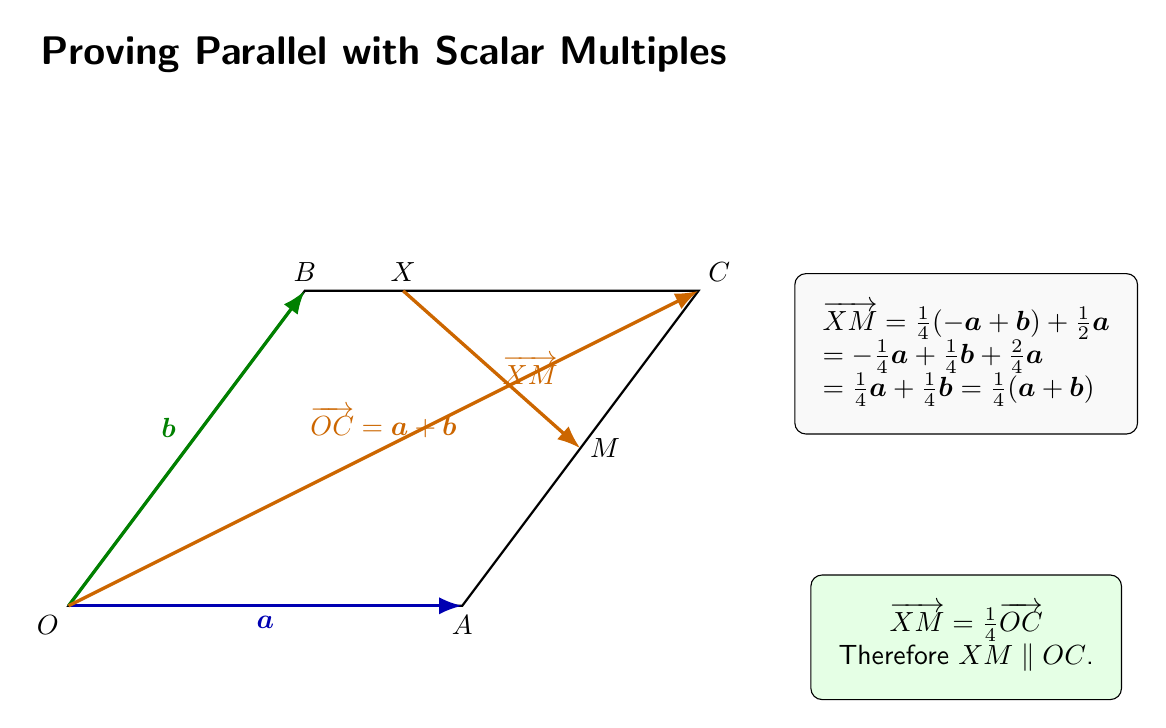
\begin{tikzpicture}[>=Latex,every node/.style={font=\sffamily},edge/.style={thick},avec/.style={->,very thick,blue!70!black},bvec/.style={->,very thick,green!50!black},proofvec/.style={->,very thick,orange!80!black}]
\node[font=\sffamily\bfseries\Large] at (0,5) {Proving Parallel with Scalar Multiples};
\coordinate (O) at (-4,-2);\coordinate (A) at (1,-2);\coordinate (B) at (-1,2);\coordinate (C) at (4,2);\coordinate (X) at (.25,2);\coordinate (M) at (2.5,0);
\draw[edge] (O)--(A)--(C)--(B)--cycle;
\node[below left] at (O) {$O$};\node[below] at (A) {$A$};\node[above] at (B) {$B$};\node[above right] at (C) {$C$};\node[above] at (X) {$X$};\node[right] at (M) {$M$};
\draw[avec] (O)--node[below] {$\bm a$}(A);\draw[bvec] (O)--node[above left] {$\bm b$}(B);\draw[proofvec] (O)--node[above] {$\overrightarrow{OC}=\bm a+\bm b$}(C);\draw[proofvec] (X)--node[right] {$\overrightarrow{XM}$}(M);
\node[draw,rounded corners,fill=gray!5,align=left,inner sep=10pt] at (7.4,1.2) {$\overrightarrow{XM}=\frac14(-\bm a+\bm b)+\frac12\bm a$\\$=-\frac14\bm a+\frac14\bm b+\frac24\bm a$\\$=\frac14\bm a+\frac14\bm b=\frac14(\bm a+\bm b)$};
\node[draw,rounded corners,fill=green!10,align=center,inner sep=10pt] at (7.4,-2.4) {$\overrightarrow{XM}=\frac14\overrightarrow{OC}$\\Therefore $XM\parallel OC$.};
\end{tikzpicture}

\end{document}
